\documentclass{beamer}
\usetheme{tokitex}

\usepackage{graphics}
\usepackage{multirow}
\usepackage{tabto}

\usepackage[english,bahasa]{babel}
\newtranslation[to=bahasa]{Section}{Bagian}
\newtranslation[to=bahasa]{Subsection}{Subbagian}

\usepackage{listings, lstautogobble}
\usepackage{color}

\definecolor{dkgreen}{rgb}{0,0.6,0}
\definecolor{gray}{rgb}{0.5,0.5,0.5}
\definecolor{mauve}{rgb}{0.58,0,0.82}

\lstset{frame=tb,
  language=pascal,
  aboveskip=1mm,
  belowskip=1mm,
  showstringspaces=false,
  columns=fullflexible,
  keepspaces=true,
  basicstyle={\small\ttfamily},
  numbers=none,
  numberstyle=\tiny\color{gray},
  keywordstyle=\color{blue},
  commentstyle=\color{dkgreen},
  stringstyle=\color{mauve},
  breaklines=true,
  breakatwhitespace=true,
  autogobble=true
}

\title{Pengenalan rekursi}
\author{Tim Olimpiade Komputer Indonesia}
\date{}

\begin{document}

\begin{frame}
\titlepage
\end{frame}

\begin{frame}
\frametitle{Pendahuluan}
Melalui dokumen ini, kalian akan:
\begin{itemize}
  \item Memahami konsep rekursi.
  \item Mempelajari rekursi sederhana.
\end{itemize}
\end{frame}

\begin{frame}
\frametitle{Pengenalan Rekursi}
\begin{itemize}
  \item Rekursi adalah keadaan yang mana sebuah fungsi menyelesaikan sebuah permasalahan dengan cara memanggil diri sendiri secara berulang kali.
  \item Jika masalah sudah cukup kecil, maka fungsi rekursi dapat langsung menghasilkan jawaban.
  \item Jika masalah terlalu besar, maka fungsi akan memanggil diri sendiri dengan cakupan masalah yang lebih kecil.
\end{itemize}
\end{frame}

\begin{frame}
\frametitle{Mengapa Perlu Ada Rekursi}
\begin{itemize}
  \item Banyak permasalahan yang lebih mudah diselesaikan (dan pendek kodenya) jika menggunakan pendekatan rekursif.
  \item Pada dasarnya, strategi iteratif (misalnya dengan \textit{for loop}) dan rekursif sama-sama melakukan sesuatu yang berulang-ulang. 
  \item Namun, terkadang solusi iteratif  untuk suatu masalah sangat sulit untuk dipikirkan dan memerlukan teknik khusus.
  \item Dengan solusi rekursif, mungkin saja lebih mudah untuk melihat dan merancang alur penyelesaiannya.
\end{itemize}
\end{frame}

\begin{frame}
\frametitle{Strategi Rekursif}
Terdapat dua hal yang perlu dipikirkan ketika menggunakan strategi rekursif:
\begin{itemize}
  \item \textit{Base case}
  
  Apa kasus paling sederhana dari permasalahan ini?
  
  \item \textit{Recurrence relation}
  
  Bagaimana hubungan rekursif dari persoalan ini dengan persoalan serupa yang lebih kecil?
\end{itemize}
\end{frame}

\begin{frame}
\frametitle{Contoh Soal: Faktorial}
Deskripsi:
\begin{itemize}
  \item Pak Dengklek baru mempelajari konsep matematika baru, yaitu faktorial.
  \item Operasi faktorial pada $N$, atau ditulis dengan notasi $N$!, adalah operasi mengalikan bilangan dari 1 sampai dengan $N$.
  \item Contoh: Jika $N = 4$, maka $4! = 1 \times 2 \times 3 \times 4 = 24$
  \item Diberikan $N$, bantu Pak Dengklek mencari hasil $N$!
\end{itemize}
\end{frame}

\begin{frame}
\frametitle{Contoh Soal: Faktorial (lanj.) }
Format masukan:
\begin{itemize}
  \item Sebuah baris berisi sebuah bilangan $N$
\end{itemize}
Format keluaran:
\begin{itemize}
  \item Sebuah baris berisi hasil $N$!
\end{itemize}
Batasan:
\begin{itemize}
  \item $1 \le N \le 10$
\end{itemize}
\end{frame}

\begin{frame}
\frametitle{Solusi}
\begin{itemize}
  \item Ide 1:
  \begin{itemize}
    \item Cukup gunakan \textit{for loop} biasa
    \item Solusi ini bekerja secara iteratif.
  \end{itemize}
  \item Ide 2: Rekursi 
\end{itemize}
\end{frame}

\begin{frame}[fragile]
\frametitle{Contoh Solusi Iteratif}
Implementasi solusi secara iteratif cukup sederhana:
\begin{lstlisting}    
  function faktorial(x: longint): longint;
  var
    jawaban: longint;
  begin
    jawaban := 1; 
    for i := 1 to x do begin
      jawaban := jawaban * i;
    end;
    
    faktorial := jawaban;
  end;
\end{lstlisting}
\end{frame}

\begin{frame}
\frametitle{Solusi Rekursif}
\textit{Base Case}
\begin{itemize}
  \item Pada batasan soal, nilai $N$ berkisar antara 1 sampai dengan 10.
  \item Dari batasan tersebut, kasus terkecilnya adalah $N=1$.
  \item Jadi $N=1$ adalah \textit{base case}, dan memang jelas diketahui bahwa 1! = 1.
\end{itemize}
\end{frame}

\begin{frame}
\frametitle{Solusi Rekursif (lanj.) }
\textit{Recurrence Relation}
\begin{itemize}
  \item Bagaimana jika $N > 1$?
  \item Untuk mencari $N!$, kita bisa mencari $(N-1)!$ dan mengalikannya dengan $N$.
  \item Jadi persoalan mencari $N!$ bisa diselesaikan dengan mudah jika diketahui $(N-1)!$.
  \item Dengan observasi ini, kita mengetahui hubungan rekursif dari $N!$. 
\end{itemize}
\end{frame}

\begin{frame}[fragile]
\frametitle{Contoh Solusi: faktorial\_rekursif.pas}
Berikut implementasi pencarian faktorial secara rekursif:
\begin{lstlisting}
  function faktorial(x: longint): longint;
  begin
    if (x = 1) then begin
      faktorial := 1
    end else begin
      faktorial := x * faktorial(x-1); 
    end;
  end;
\end{lstlisting}
\end{frame}

\begin{frame}[fragile]
\frametitle{Contoh Solusi: faktorial\_rekursif.pas (lanj.)}
Pemanggilan pada program utama bisa dilakukan seperti memanggil fungsi biasa:
\begin{lstlisting}
  ...
  
  begin
    writeln('4! = ', faktorial(4));
  end.
\end{lstlisting}
\end{frame}

\begin{frame}
\frametitle{Contoh Eksekusi Fungsi}
\begin{columns}
  \column{0.38\linewidth}
    \centering
    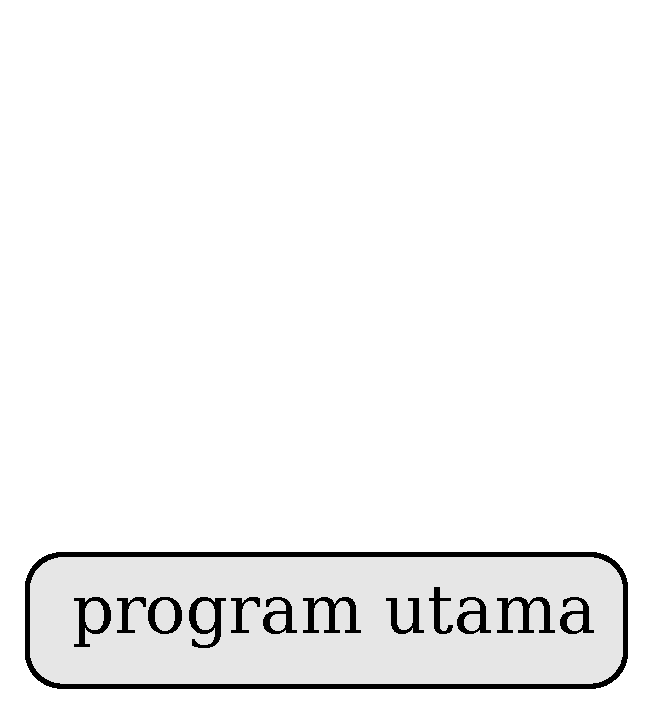
\includegraphics[width=4cm]{asset/rekursi-1.pdf}
  \column{0.58\linewidth}
    \begin{itemize}
      \item Pada awalnya, program utama dijalankan. Misalkan hendak dicari nilai $4!$.
    \end{itemize} 
  \end{columns} 
\end{frame}

\begin{frame}
\frametitle{Contoh Eksekusi Fungsi (lanj.)}
\begin{columns}
  \column{0.38\linewidth}
    \centering
    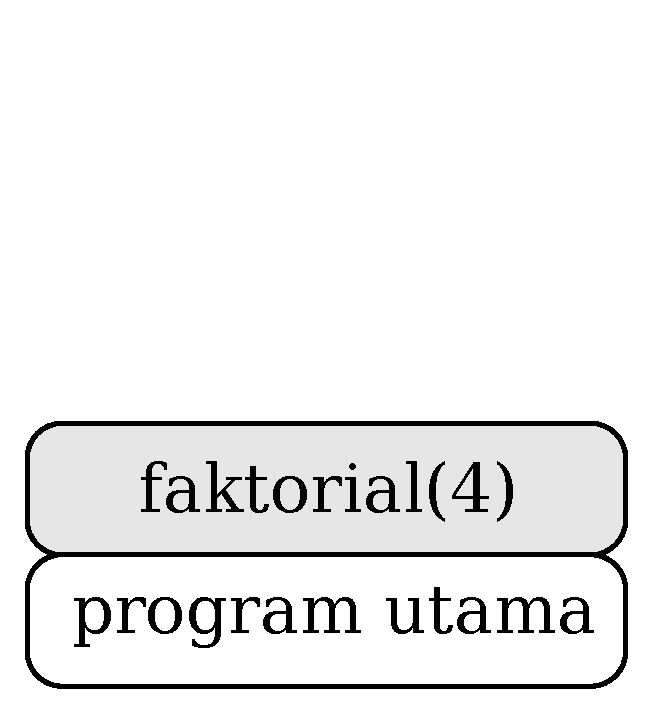
\includegraphics[width=4cm]{asset/rekursi-2.pdf}
  \column{0.58\linewidth}
    \begin{itemize}
      \item Dari program utama, dipanggil fungsi \textbf{faktorial(4)}.
      \item Pada saat ini, status program utama adalah "tidak aktif", dan akan "aktif" kembali setelah fungsi \textbf{faktorial(4)} selesai.
    \end{itemize}
  \end{columns} 
\end{frame}

\begin{frame}
\frametitle{Contoh Eksekusi Fungsi (lanj.)}
\begin{columns}
  \column{0.38\linewidth}
    \centering
    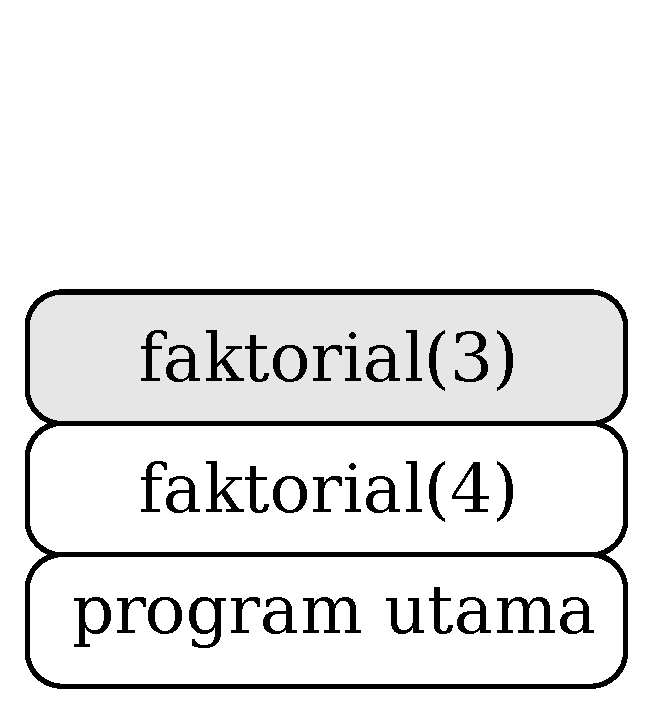
\includegraphics[width=4cm]{asset/rekursi-3.pdf}
  \column{0.58\linewidth}
    \begin{itemize}
      \item \textbf{faktorial(4)} mengeksekusi baris "faktorial := x * faktorial(x-1)", yang pada kasus ini \textbf{x} = 4.
      \item Akibatnya, dipanggil fungsi \textbf{faktorial(3)}. 
      \item Kini yang "aktif" adalah \textbf{faktorial(3)}.
    \end{itemize}
  \end{columns} 
\end{frame}

\begin{frame}
\frametitle{Contoh Eksekusi Fungsi (lanj.)}
\begin{columns}
  \column{0.38\linewidth}
    \centering
    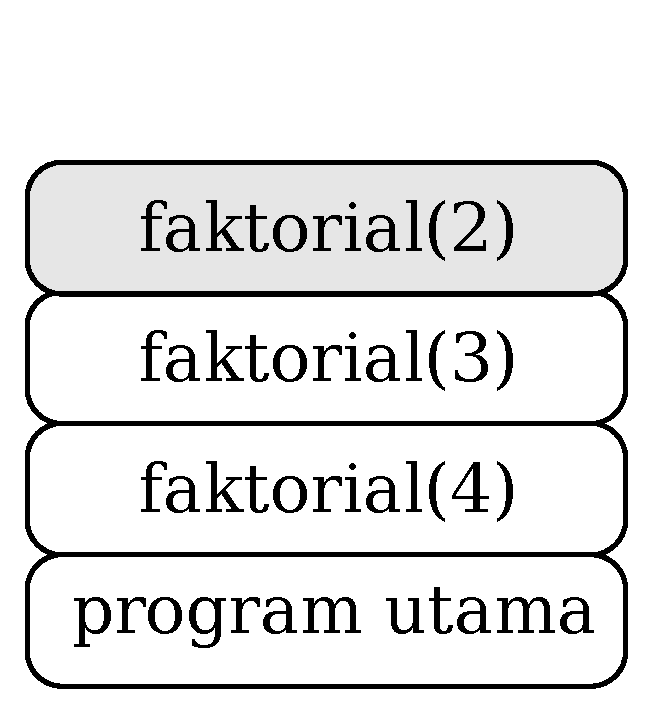
\includegraphics[width=4cm]{asset/rekursi-4.pdf}
  \column{0.58\linewidth}
    \begin{itemize}
      \item Hal serupa terjadi untuk mencari nilai \textbf{faktorial(3)}.
    \end{itemize}
  \end{columns} 
\end{frame}

\begin{frame}
\frametitle{Contoh Eksekusi Fungsi (lanj.)}
\begin{columns}
  \column{0.38\linewidth}
    \centering
    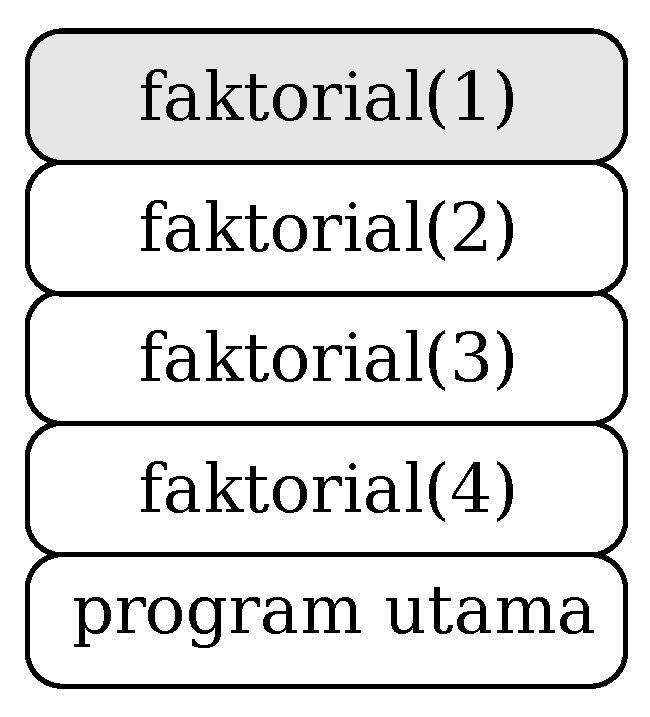
\includegraphics[width=4cm]{asset/rekursi-5.pdf}
  \column{0.58\linewidth}
    \begin{itemize}
      \item Terjadi juga untuk mencari nilai \textbf{faktorial(2)}.
    \end{itemize}
  \end{columns} 
\end{frame}

\begin{frame}
\frametitle{Contoh Eksekusi Fungsi (lanj.)}
\begin{columns}
  \column{0.38\linewidth}
    \centering
    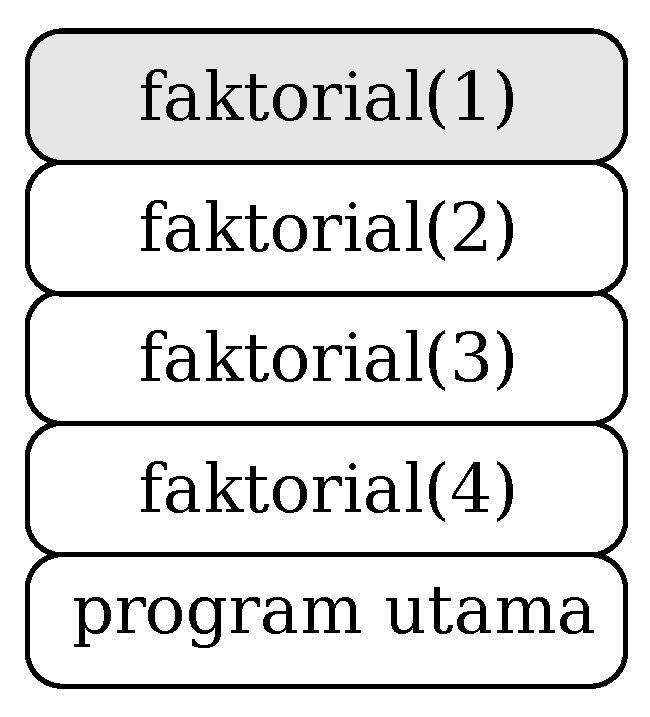
\includegraphics[width=4cm]{asset/rekursi-5.pdf}
  \column{0.58\linewidth}
    \begin{itemize}
      \item Pada saat ini, \textbf{faktorial(1)} tidak lagi melakukan pemanggilan rekursif, berhubung ditemui \textit{base case}.
      \item Sebaliknya, langsung dikembalikan nilai 1 sebagai jawaban atas \textbf{faktorial(1)}.
    \end{itemize}
  \end{columns} 
\end{frame}

\begin{frame}
\frametitle{Contoh Eksekusi Fungsi (lanj.)}
\begin{columns}
  \column{0.38\linewidth}
    \centering
    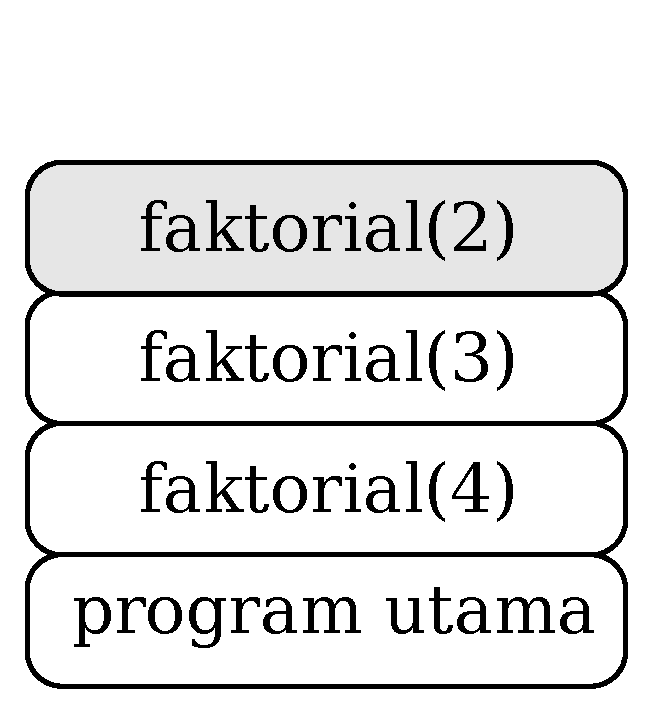
\includegraphics[width=4cm]{asset/rekursi-4.pdf}
  \column{0.58\linewidth}
    \begin{itemize}
      \item \textbf{faktorial(1)} selesai, kini kembali ke \textbf{faktorial(2)}.
      \item Nilai \textbf{faktorial(2)} kini ditemukan, yaitu 2 $\times$ \textbf{faktorial(1)}.
      \item Fungsi \textbf{faktorial(2)} mengembalikan nilai 2 ke pemanggilnya, lalu selesai.
    \end{itemize}
  \end{columns} 
\end{frame}

\begin{frame}
\frametitle{Contoh Eksekusi Fungsi (lanj.)}
\begin{columns}
  \column{0.38\linewidth}
    \centering
    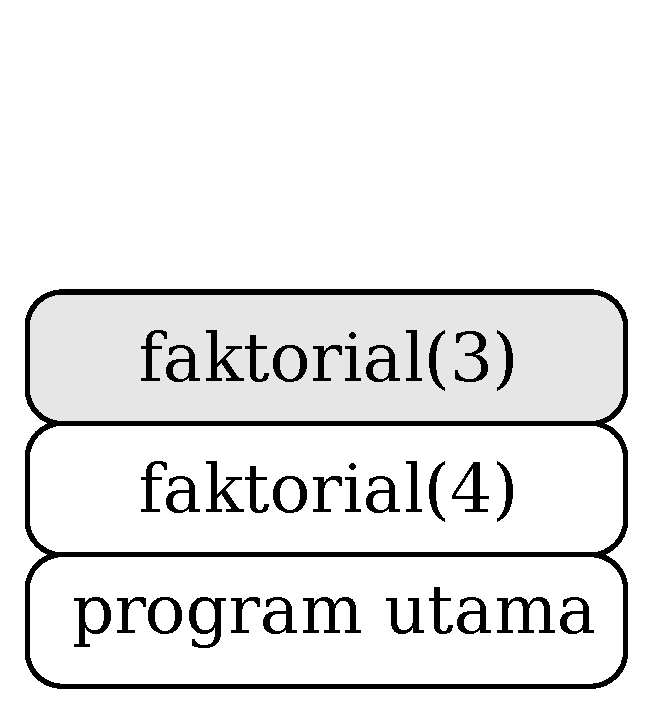
\includegraphics[width=4cm]{asset/rekursi-3.pdf}
  \column{0.58\linewidth}
    \begin{itemize}
      \item Setelah menerima nilai kembalian \textbf{faktorial(2)}, \textbf{faktorial(3)} kembali aktif.
      \item Hasilnya dapat ditemukan, yaitu \\ 3 $\times$ \textbf{faktorial(2)}.
      \item Fungsi \textbf{faktorial(3)} mengembalikan nilai 6 ke pemanggilnya, lalu selesai.
    \end{itemize}
  \end{columns} 
\end{frame}

\begin{frame}
\frametitle{Contoh Eksekusi Fungsi (lanj.)}
\begin{columns}
  \column{0.38\linewidth}
    \centering
    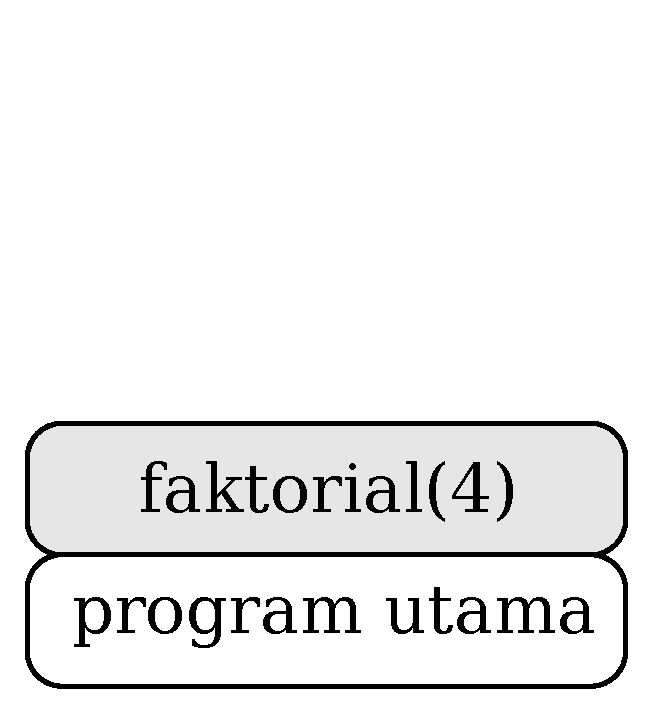
\includegraphics[width=4cm]{asset/rekursi-2.pdf}
  \column{0.58\linewidth}
    \begin{itemize}
      \item Kini \textbf{faktorial(4)} kembali aktif.
      \item Hasilnya dapat ditemukan, yaitu \\ 4 $\times$ \textbf{faktorial(3)}.
      \item Fungsi \textbf{faktorial(4)} mengembalikan nilai 24 ke pemanggilnya, lalu selesai.
    \end{itemize}
  \end{columns} 
\end{frame}

\begin{frame}
\frametitle{Contoh Eksekusi Fungsi (lanj.)}
\begin{columns}
  \column{0.38\linewidth}
    \centering
    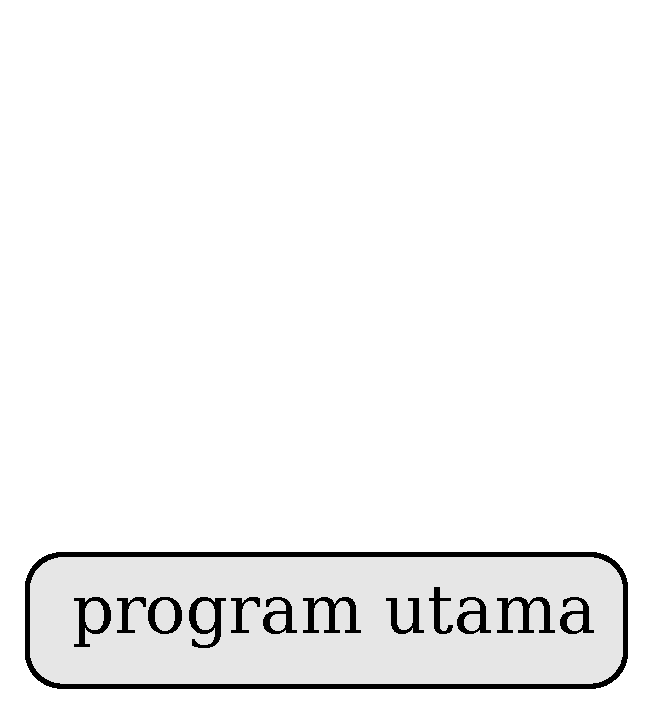
\includegraphics[width=4cm]{asset/rekursi-1.pdf}
  \column{0.58\linewidth}
    \begin{itemize}
      \item Program utama yang memanggil \textbf{faktorial(4)} menerima nilai kembaliannya, yaitu 24.
      \item Program utama kembali menjalankan perintah-perintah berikutnya.
    \end{itemize}
  \end{columns} 
\end{frame}

\begin{frame}
\frametitle{Kompleksitas Solusi}
\begin{itemize}
  \item Baik secara iteratif maupun rekursif, kompleksitasnya adalah $O(N)$.
  \item Setiap pemanggilan rekursif membutuhkan alokasi memori, sehingga jika pemanggilannya semakin dalam, semakin banyak tambahan memori yang digunakan.
  \item Waktu untuk mengalokasikan memori juga menyebabkan solusi rekursif cenderung bekerja lebih lambat dibandingkan solusi iteratif.
\end{itemize}
\end{frame}

\begin{frame}
\frametitle{Materi Selanjutnya}
\begin{itemize}
  \item Pada pembelajaran ini, rekursi yang digunakan masih sangat sederhana.
  \item Bahkan belum terasa bahwa solusi rekursi lebih mudah dan pendek kodenya dibandingkan solusi iteratif.
  \item Pembelajaran selanjutnya tentang rekursi yang lebih kompleks akan menunjukkan hal tersebut.
\end{itemize}
\end{frame}

\end{document}
